\documentclass[tikz,border=5pt]{standalone}
\usepackage[T1]{fontenc}
\usepackage{lmodern,amsmath,amssymb}
\usetikzlibrary{arrows.meta,calc,positioning,fit,backgrounds,shapes.geometric,matrix,decorations.pathreplacing,patterns}
\definecolor{ink}{gray}{0.08}
\definecolor{wash}{gray}{0.965}
\definecolor{soft}{gray}{0.45}
\tikzset{box/.style={draw=ink,line width=.65pt,fill=white,align=center,inner sep=4pt,outer sep=0pt,font=\small},flow/.style={draw=ink,line width=.65pt,-{Latex[length=1.8mm,width=1.3mm]},rounded corners=2pt},annotation/.style={font=\scriptsize,text=soft,align=center},groupbox/.style={draw=soft,dashed,line width=.45pt,fill=wash}}
\begin{document}
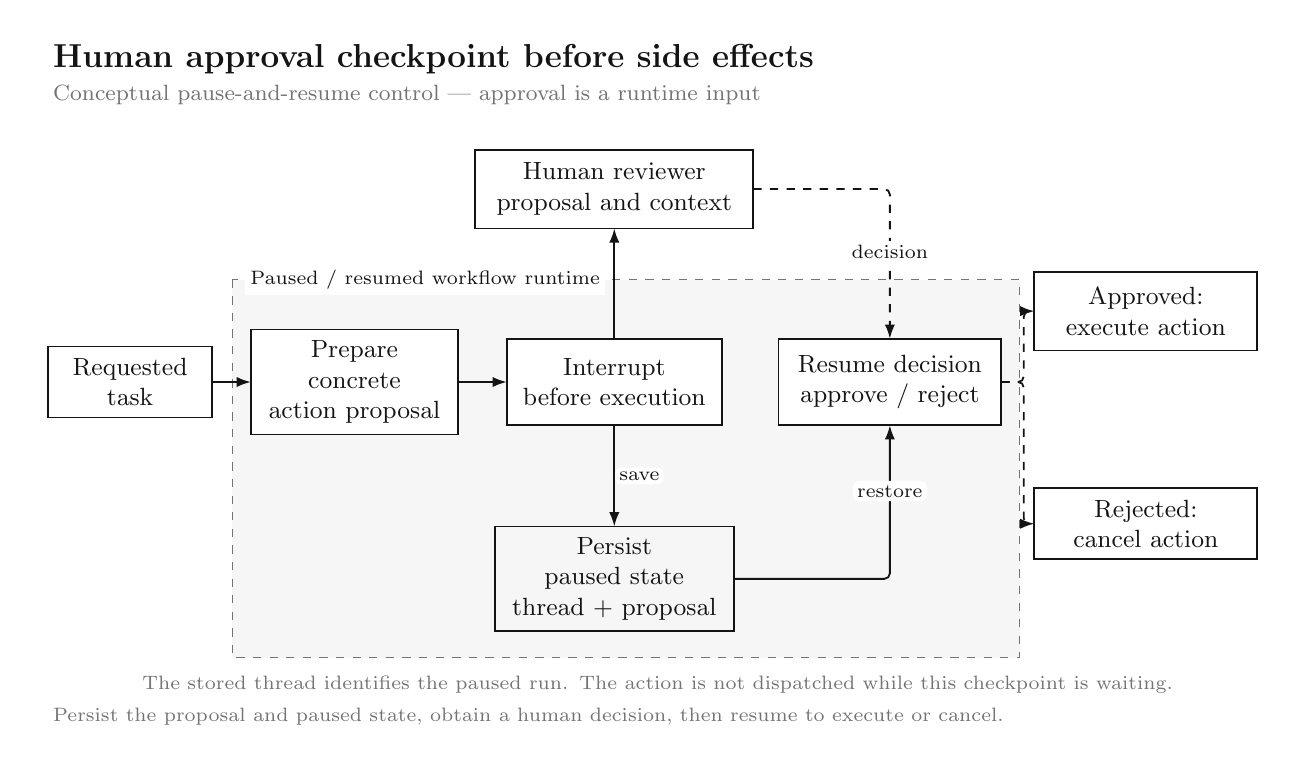
\begin{tikzpicture}[x=1cm,y=-1cm,font=\rmfamily,text=ink]

\path[use as bounding box] (0,0) rectangle (16,9);
\node[anchor=west,font=\large\bfseries] at (.2,.4) {Human approval checkpoint before side effects};
\node[anchor=west,font=\footnotesize,text=soft] at (.2,.85) {Conceptual pause-and-resume control | approval is a runtime input};
\begin{pgfonlayer}{background}
\draw[groupbox] (2.6,3.2) rectangle (12.6,8.0);
\node[anchor=west,font=\scriptsize,fill=white,inner sep=2pt] at (2.75,3.2) {Paused / resumed workflow runtime};
\end{pgfonlayer}
\node[box,minimum width=2.05cm,minimum height=0.9cm,text width=1.7999999999999998cm] (request) at (1.3,4.5) {Requested task};
\node[box,minimum width=2.6cm,minimum height=1.1cm,text width=2.35cm] (proposal) at (4.15,4.5) {Prepare concrete\\action proposal};
\node[box,minimum width=2.7cm,minimum height=1.1cm,text width=2.45cm] (pause) at (7.45,4.5) {Interrupt\\before execution};
\node[box,minimum width=3.5cm,minimum height=1.0cm,text width=3.25cm] (reviewer) at (7.45,2.05) {Human reviewer\\proposal and context};
\node[box,minimum width=2.8cm,minimum height=1.1cm,text width=2.55cm] (resume) at (10.95,4.5) {Resume decision\\approve / reject};
\node[box,fill=wash,minimum width=3.0cm,minimum height=1.1cm,text width=2.75cm] (state) at (7.45,7.0) {Persist paused state\\thread + proposal};
\node[box,minimum width=2.8cm,minimum height=1.0cm,text width=2.55cm] (execute) at (14.2,3.6) {Approved:\\execute action};
\node[box,minimum width=2.8cm,minimum height=0.9cm,text width=2.55cm] (cancel) at (14.2,6.3) {Rejected:\\cancel action};
\begin{pgfonlayer}{background}
\draw[flow] (request.east) -- (proposal.west);
\draw[flow] (proposal.east) -- (pause.west);
\draw[flow] (pause.north) -- (reviewer.south);
\draw[flow] (pause.south) -- (state.north) node[midway,right,fill=white,inner sep=1.5pt,font=\scriptsize] {save};
\draw[flow,dashed] (reviewer.east) -- (10.95,2.05) -- (resume.north) node[midway,above,fill=white,inner sep=1.5pt,font=\scriptsize] {decision};
\draw[flow] (state.east) -- (10.95,7.0) -- (resume.south) node[midway,above,fill=white,inner sep=1.5pt,font=\scriptsize] {restore};
\draw[flow,dashed] (resume.east) -- (12.65,4.5) -- (12.65,3.6) -- (execute.west);
\draw[flow,dashed] (resume.east) -- (12.65,4.5) -- (12.65,6.3) -- (cancel.west);
\end{pgfonlayer}
\node[annotation,anchor=center,text width=14cm] at (8.0,8.35) {The stored thread identifies the paused run. The action is not dispatched while this checkpoint is waiting.};
\node[anchor=west,align=left,font=\scriptsize,text=soft,text width=15.6cm] at (.2,8.75) {Persist the proposal and paused state, obtain a human decision, then resume to execute or cancel.};
\end{tikzpicture}
\end{document}
